%% 3章用 (Grid)

前述の理論に基づき，本研究ではGo言語を用いてRemesアルゴリズムを実装した．
以下の図表は，関数 $f(x) = \frac{1}{1+25x^2}$ ($n=15$) を近似した際の収束過程を示したものである．

表\ref{tab:remes-grid-log}は，各反復で算出された参照均等誤差 $|E|$ と，その時点での誤差関数の極値の絶対値の最大値と最小値の差（Deviation）の推移を示したものである．

本実装における収束判定条件は，すべてのパラメータの変化量が機械イプシロン（$\epsilon_{\text{mach}} \approx 2.22 \times 10^{-16}$）以下になった時点とする．
\begin{itemize}
  \item 近似多項式の係数ベクトル $\boldsymbol{c}$ の最大変化量：
  \[ \|\boldsymbol{c}^{(k+1)} - \boldsymbol{c}^{(k)}\|_\infty \le \epsilon_{\text{mach}}. \]
  \item 参照点ベクトル $\boldsymbol{\xi}$ の最大変化量：
  \[ \|\boldsymbol{\xi}^{(k+1)} - \boldsymbol{\xi}^{(k)}\|_\infty \le \epsilon_{\text{mach}}. \]
  \item 均等誤差パラメータ $E$ の変化量：
  \[ |E^{(k+1)} - E^{(k)}| \le \epsilon_{\text{mach}}. \]
\end{itemize}
これにより，数値計算上の限界精度まで解が収束したことを保証する．

表中の Deviation は，係数が収束に向かうにつれて交替定理の条件（等振幅性）が満たされていく様子を表す指標であり，理論通り急速に 0 に収束していることが確認できる．

図\ref{fig:remes-grid-convergence}は，この Deviation の推移を可視化したものである．
初期段階では不揃いであった誤差の波形が，最終的には振幅が一定の美しい等振動波形へと収束していることが見て取れる．

\begin{figure}[H]
 \centering
 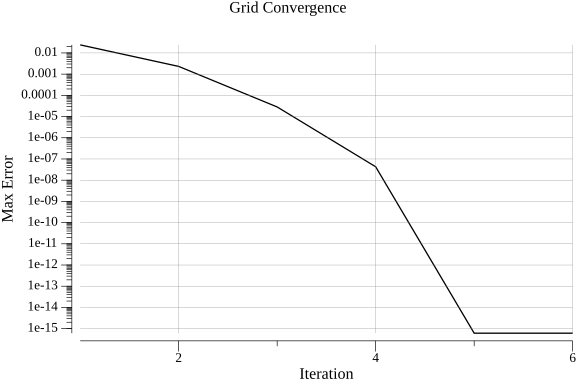
\includegraphics[width=0.6\linewidth]{material/remes/outputs/grid/convergence_grid.png}
 \caption{グリッド極値点探索法による最大誤差の収束履歴}
 \label{fig:remes-grid-convergence}
\end{figure}

\begin{figure}[H]
 \centering
 \begin{minipage}[b]{0.48\textwidth}
  \centering
  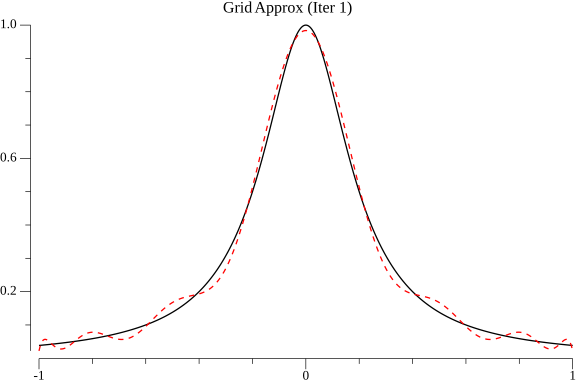
\includegraphics[width=1.0\linewidth]{material/remes/outputs/grid/func_remes_grid_iter01.png}
  \caption{Iter 1}
 \end{minipage}
 \hfill
 \begin{minipage}[b]{0.48\textwidth}
  \centering
  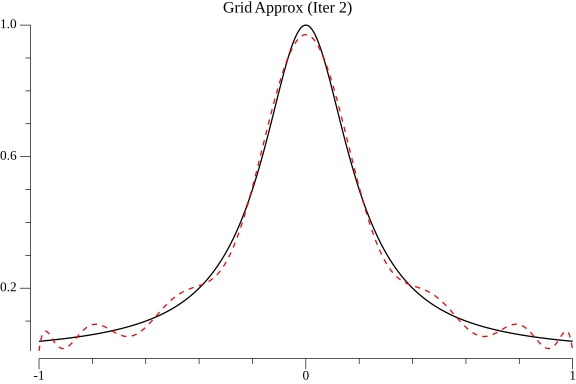
\includegraphics[width=1.0\linewidth]{material/remes/outputs/grid/func_remes_grid_iter02.png}
  \caption{Iter 2}
 \end{minipage}

 \begin{minipage}[b]{0.48\textwidth}
  \centering
  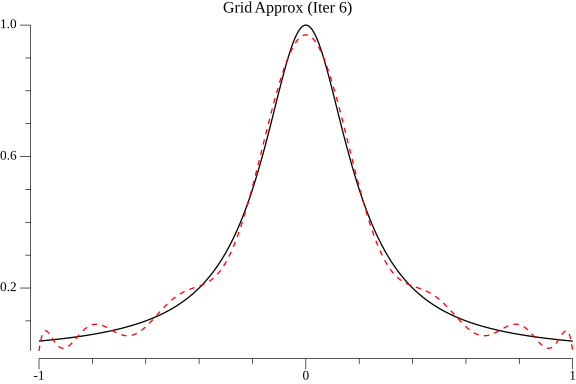
\includegraphics[width=1.0\linewidth]{material/remes/outputs/grid/func_remes_grid_iter06.png}
  \caption{Iter 6}
 \end{minipage}

 \caption{グリッド法: 近似多項式の推移}
 \label{fig:remes-grid-approx}
\end{figure}
\begin{figure}[H]
 \centering
 \begin{minipage}[b]{0.48\textwidth}
  \centering
  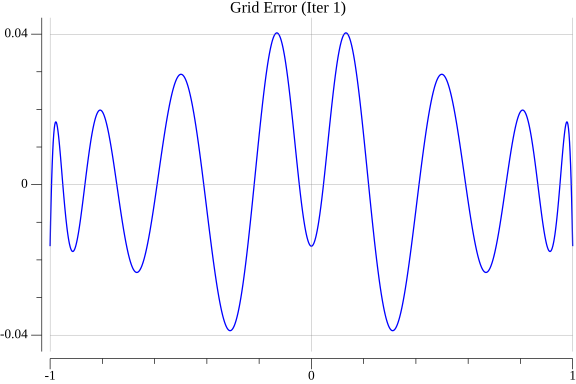
\includegraphics[width=1.0\linewidth]{material/remes/outputs/grid/error_remes_grid_iter01.png}
  \caption{Iter 1}
 \end{minipage}
 \hfill
 \begin{minipage}[b]{0.48\textwidth}
  \centering
  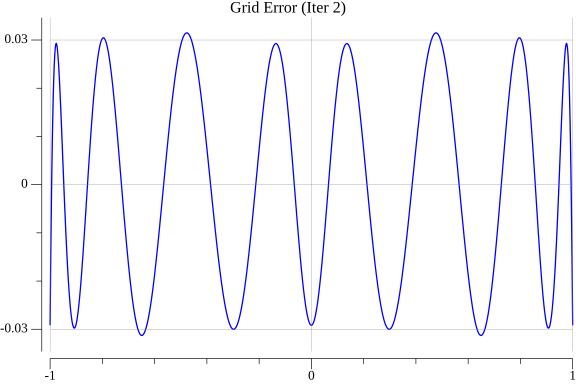
\includegraphics[width=1.0\linewidth]{material/remes/outputs/grid/error_remes_grid_iter02.png}
  \caption{Iter 2}
 \end{minipage}

 \begin{minipage}[b]{0.48\textwidth}
  \centering
  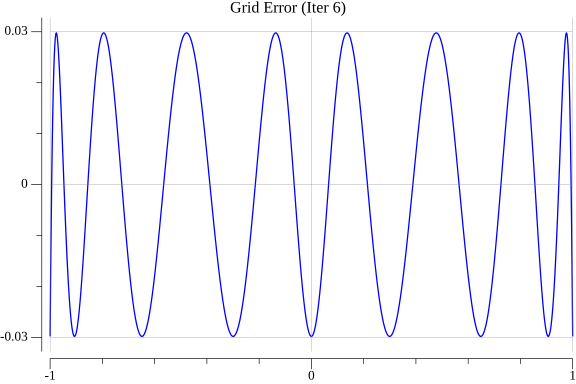
\includegraphics[width=1.0\linewidth]{material/remes/outputs/grid/error_remes_grid_iter06.png}
  \caption{Iter 6}
 \end{minipage}

 \caption{グリッド法: 誤差関数の推移}
 \label{fig:remes-grid-error}
\end{figure}

\begin{table}[H]
 \centering
 \caption{グリッド極値点探索法の収束ログ}
 \label{tab:remes-grid-log}
 \begin{tabular}{crrrr}
 \toprule
 Iter & $|E|$ & Coeff Norm & Node Move & Error Change \\
 \midrule
 1 & $1.63552e-02$ & $0.00000e+00$ & $0.00000e+00$ & $0.00000e+00$ \\
 2 & $2.91689e-02$ & $1.37847e-02$ & $4.92138e-02$ & $1.28137e-02$ \\
 3 & $2.97722e-02$ & $1.25091e-03$ & $3.16228e-03$ & $6.03335e-04$ \\
 4 & $2.97756e-02$ & $1.30728e-05$ & $1.41421e-03$ & $3.38844e-06$ \\
 5 & $2.97756e-02$ & $1.90384e-08$ & $0.00000e+00$ & $7.83719e-09$ \\
 6 & $2.97756e-02$ & $0.00000e+00$ & $0.00000e+00$ & $0.00000e+00$ \\
 \bottomrule
 \end{tabular}
\end{table}

\begin{table}[H]
 \centering
 \caption{グリッド極値点探索結果の等振幅性確認（節点近傍の偏差）}
 \label{tab:remes-grid-final-check}
 \begin{tabular}{crrr}
 \toprule
 No. & Grid誤差 & Brent誤差 & 差分 \\
 \midrule
 1 & $2.97755952e-02$ & $2.97755952e-02$ & $-6.86950e-16$ \\
 2 & $2.97755952e-02$ & $2.97755952e-02$ & $3.80066e-11$ \\
 3 & $2.97755952e-02$ & $2.97755952e-02$ & $1.63316e-11$ \\
 4 & $2.97755952e-02$ & $2.97755952e-02$ & $1.94925e-12$ \\
 5 & $2.97755952e-02$ & $2.97755952e-02$ & $4.93021e-12$ \\
 6 & $2.97755952e-02$ & $2.97755952e-02$ & $1.21936e-12$ \\
 7 & $2.97755952e-02$ & $2.97755952e-02$ & $4.76352e-12$ \\
 8 & $2.97755952e-02$ & $2.97755952e-02$ & $6.46216e-12$ \\
 9 & $2.97755952e-02$ & $2.97755952e-02$ & $0.00000e+00$ \\
 10 & $2.97755952e-02$ & $2.97755952e-02$ & $6.46216e-12$ \\
 11 & $2.97755952e-02$ & $2.97755952e-02$ & $4.76358e-12$ \\
 12 & $2.97755952e-02$ & $2.97755952e-02$ & $1.21927e-12$ \\
 13 & $2.97755952e-02$ & $2.97755952e-02$ & $4.93020e-12$ \\
 14 & $2.97755952e-02$ & $2.97755952e-02$ & $1.94927e-12$ \\
 15 & $2.97755952e-02$ & $2.97755952e-02$ & $1.63316e-11$ \\
 16 & $2.97755952e-02$ & $2.97755952e-02$ & $3.80066e-11$ \\
 17 & $2.97755952e-02$ & $2.97755952e-02$ & $-1.34615e-15$ \\
 \bottomrule
 \end{tabular}
\vspace{1mm}

\small \textbf{注：}
\small 上表は，区間 $[-1.0,1.0]$ を探索するRemesアルゴリズムによって導かれた誤差関数に対する表である．

\small Grid誤差とはBrent法をもちいることで極値点探索を行ったRemesアルゴリズムで導出された誤差関数の各極値点で観測された誤差である．

\small Brent誤差とはBrent法という極値点探索アルゴリズムにより観測された誤差の絶対値である．

\[
 \text{観測された最大誤差} \; \|E\|_{\max}^{\text{strict}}(f) = \max_{x \in [-1.0,1.0]} |f(x) - p^*(x)| \approx 2.97811342e-02 .
 \]
\end{table}
